
\section{Pebble failure modeling}
\label{failureDiscussion}
%In modeling pebble failure, there are two main tasks. The first is to develop a model for predicting a pebble failure event; { i.e.} what load (mechanical or thermal) will cause a pebble to crack, shatter, fracture, etc. The second is to develop a model which simulates the failure of that pebble; { i.e.} a scheme to treat a cracked, shattered, or crushed pebble in the assembly. 

The discrete element method has been used for studies in a variety of fields for studying inter-particle forces and the homogeneously distributed force networks that arise in packed beds (for example, see Ref.~\cite{Makse2000}). The discrete element method was also used in the fusion community to attempt to model failure initiation and propagation\cite{Annabattula2012a, Zhao2012, Zhao2013}. They too observed that a relatively few number of high-force networks, distributed troughought the bed supported the external mechanical loads. The even distribution of the force networks was used to defend the development of a probability-based predictor for failure. We make use of the probability argument of Zhao, {et al.} for the current study\cite{Zhao2013}. Their basic premise is that probability distributions of strength curves for pebble crushing have been observed (see, for example crush loads of Ref.~\cite{Tsuchiya1998}). Then in DEM models, a probability distribution of inter-particle forces are also observed. Overlaying the two probabilities resulted in seemingly random locations of pebbles satisfying the failure criteria -- not strictly along the high-force chains running through packed beds.

We apply the theory of Zhao, { et al.} in the following manner. If pebbles fail at random locations, we may de-couple the task of predicting pebble failure ({ i.e.} finding the mechanical or thermal load that causes a pebble to fail) from the task of modeling the ramifications of pebble failure. In our model, we begin with a starting point of a packed bed and then simply flag pebbles at random for `failing'. For our first model of failure, after a pebble has been flagged it is removed from the system entirely. The removal disrupts the meta-static state of the ensemble and the remaining pebbles re-settle. In reality, the ceramic pebbles generally break into just a few large pieces that remain in the system. Under development is a method for recreating that behavior in the DEM domain, it will be reported in future studies.

%Experiments on crushing single, brittle pebbles reveal that there are a number of failure modes\cite{Wu2004}. At one end, the pebble may simply crack and continue to hold a load for some time. At the other extreme, a pebble may crush virtually into a dust. We concern ourselves with the latter for this study. When a pebble in our simulation has been flagged for failure, we remove the pebble completely from the ensemble and then allow the remaining pebbles to rearrange to compensate for the lack of equilibrium on their contact forces. 


%\section{Simulation methods}
%\label{back} 
Our three-dimensional system consists of mono-dispersed particles of diameter $d$. The particles are constrained by two rigid walls in the $x$-direction at locations of $x = \pm 10d$  and periodic boundary conditions in the $y$-direction located at $y = \pm 7.5d$. Gravity acts in the downward $z$-direction and the particles are bound from below by a rigid wall at $z=0$. The size of the system allows approximately 10~000 particles to fill to a height of approximately $z = 30d$. The volume was chosen to represent the long, tall, narrow channels seen in many solid breeder module designs\cite{ Cho2008, Poitevin2010, Enoeda2003}.


\subsection{Material properties}
For this study, the material was chosen as lithium metatinatate with all properties coming from Ref.~\cite{Gierszewski1998}; they are summarized in Table~\ref{tab:matProps}

\begin {table}[tp] %
\caption{Maximum load and nominal tension.}
\label {tab:matProps} \centering %
\begin {tabular}{ cccccc }
\toprule %
E            &     $\nu$    &       k         &    C             &   $\alpha$                     \\
(GPa)    &                     &(W/m-K)  &  (J/kg-K)  &   (1/K)                                   \\\toprule
126       &      0.24       &  2.5          &  1156       &  $15\times10^{-6}$       \\\bottomrule
\end{tabular}
\end{table}



\subsection{Methodology}
\label{method}
\begin{figure}[t]
	\centering
	\begin{subfigure}[b]{0.23\textwidth}
		\centering
		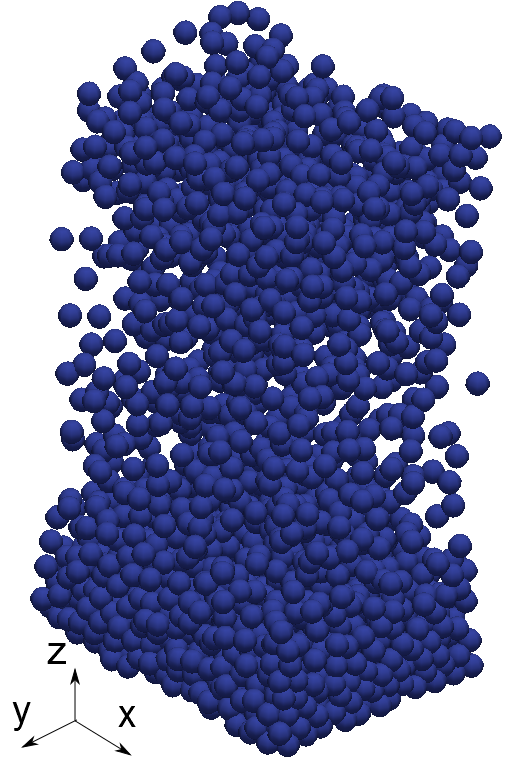
\includegraphics[width=\textwidth]{chapters/figures/fill01.png}
	\end{subfigure}
	%\begin{subfigure}[b]{0.15\textwidth}
	%	\centering
	%	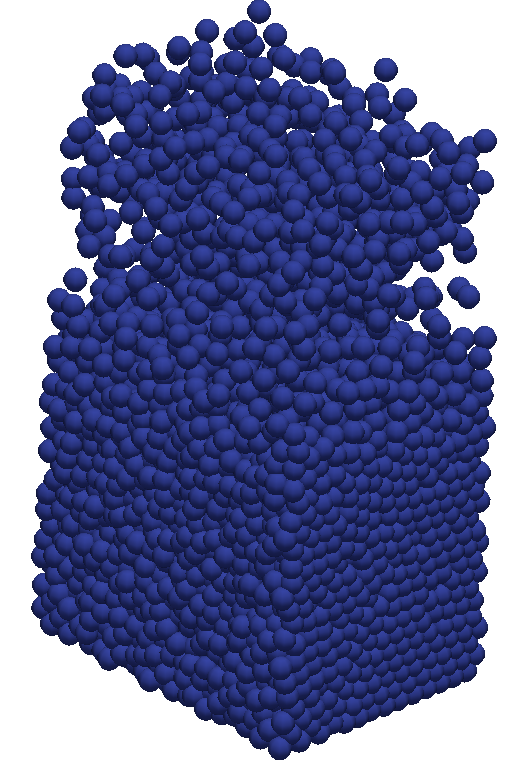
\includegraphics[width=\textwidth]{chapters/figures/fill02.png}
	%\end{subfigure}
	\begin{subfigure}[b]{0.23\textwidth}
		\centering
		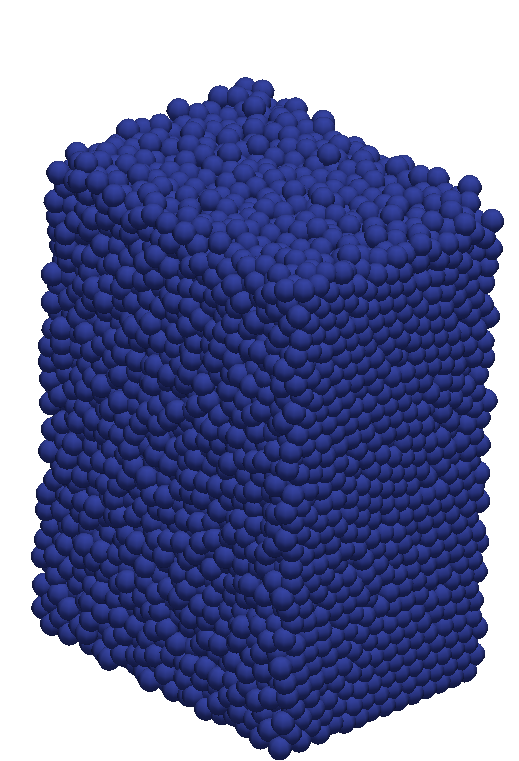
\includegraphics[width=\textwidth]{chapters/figures/fill03.png}
	\end{subfigure}
	\caption{Demonstrating the pouring process of $N = 10550$ pebbles into the control volume with an early (left) and late (right) snapshot.}
\label{fig:fill01}
\end{figure}

text

\begin{figure}[t]
	\centering
	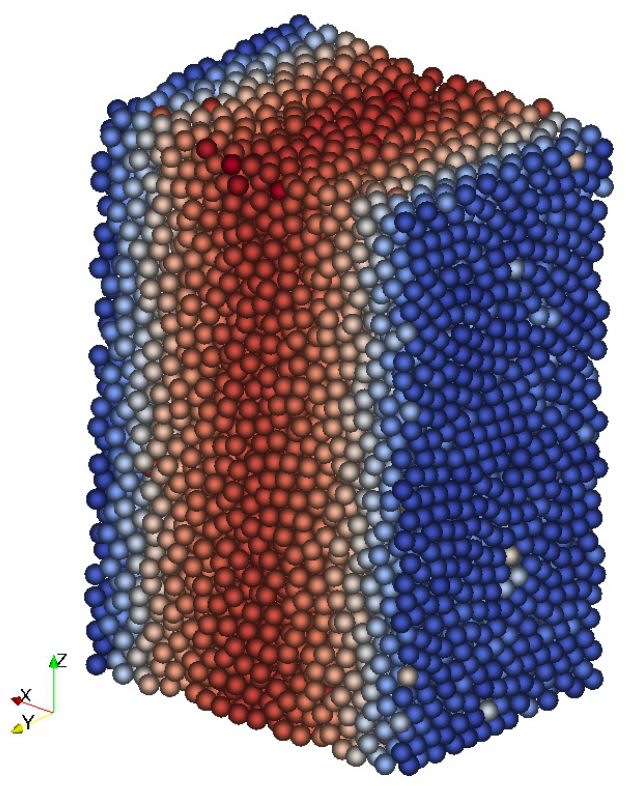
\includegraphics[trim=1cm 8cm 3cm 4cm, width=0.4\textwidth]{chapters/figures/pebbleBedTemperature}
	\caption{Temperature distribution of pebbles in the $10\%$ failed bed. At the end of steady-state heating, a one-dimensional profile is evident in all pebble beds studied here. The pebbles are receiving nuclear heating. Cooling proceeds through the pebbles in contact with the walls in the $x$-direction. [color online]}
\label{fig:pebbleBedTemperature}
\end{figure}


All the test cases begin with a common starting point of a filled, lightly packed volume of 10~550 pebbles. The pebbles are poured into the volume from above and come to rest under the influence of gravity (see Fig.~\ref{fig:fill01}). Initially, to recreate how we may pack solid breeders in reality, we attempted vibration simulations in order to pack the pebbles into a more dense state. However, we found the same packing states (from a void fraction standpoint) could be realized in a more computationally-simple manner by lowering a $z$-plane wall onto the top of the packed bed until it experienced some small force. This pour-press-packing routine was repeated many times and all the beds exhibited the same force on the top wall at roughly the same packing fraction. We took the last case, with a packing fraction (volume of $N$ pebbles per total volume) of $\phi_\text{bl}= 62.9\%$, as our baseline configuration. The packed bed state was saved and used as a starting point for numerous `failed' cases to be described later.

For the baseline case, we assigned an initial temperature of $T_\text{ref}$ to both the pebbles and the $x$ walls, then set a constant nuclear heating source on each pebble. The nuclear energy raised the temperature of the pebbles while the walls remained at $T_\text{ref}$ for cooling. The process ran until a steady state was reached (for example, see Fig.~\ref{fig:pebbleBedTemperature}); the total thermal energy of the bed, $E =\sum_i^N m_iC_i T_i$, was monitored and the simulation completed when the value was constant. At steady state, we analyzed thermomechanical characteristics of the pebble bed such as effective thermal conductivity, average coordination number, temperature profiles in the bed, and inter-particle contact forces.

As mentioned in Sec.~\ref{failureDiscussion}, in this study we model pebble failure without considering the cause of failure. This is done by randomly selecting pebbles from the ensemble, regardless of forces acting upon the pebble, and removing them entirely. When a pebble is removed, the neighboring pebbles react due to the imbalance of forces and the bed settles into a new configuration. We differentiated the failed beds by their percentage of failed pebbles: $\eta = $ number of failed pebbles per original ensemble size. After failing we again applied our heating routine.